Un tanque de $100\,\mathrm L$ contiene inicialmente $50\,\mathrm L$ de agua pura. Entra disolución de $0.1\,\mathrm{kg/L}$ a $4\,\mathrm{L/min}$ y sale mezcla a $2\,\mathrm{L/min}$ por una tubería. Cuando el tanque se llena, el exceso sale por un rebosadero. Suponga mezcla perfecta y volúmenes aditivos. Formule los balances de cada régimen y determine la cantidad de sal $S(t)$ para $t\ge0$.

\Needspace{5.61cm}
\begin{center}
\begin{minipage}{\linewidth}
\centering
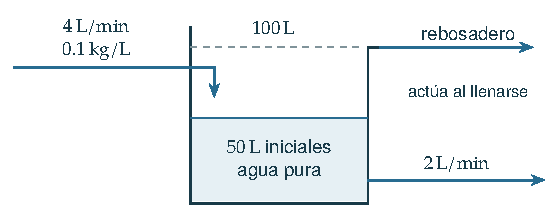
\includegraphics[width=10.59cm]{assets/M2-E0031-setup.pdf}\par
\smallskip{\small Tubería de salida y rebosadero del depósito.\par}
\end{minipage}
\end{center}
